%************************************************
\chapter{Introduction}\label{ch:introduction}
%************************************************
\section{Modeling the Language}
We discuss here the origin of the notion of \textit{language model} and why calling
such systems as that rises important questions on the longstanding debate between
formalists and cognitivist and corpus-based linguistics. We then discuss recent
studies on linguistics properties encoded in language models. 
We then present the Transformer as probably the best machine language and knowledge learner
in that each component of the systems seems to learn different properties of the language
and human knowledge broadly.
We then propose the claims and work of the thesis.
\subsection{A dialog between Shannon and Chomsky}
It is curious that we still don't know where the expression \textit{language model} come from and when it etablishes. Not the notion of what is a \textit{language model} but the expression itself. Because for the notion, we know that the idea of language model is quite old and one of the earliest 
formulations closely related to what we now call language modeling can be found in Shannon's 
work on information theory~\citet{shannon1948mathematical}. 
Shannon starts from a simple observation: sequences of linguistic symbols are not random, 
but exhibit regularities characteristic of the language.
\begin{quote}
    \small\itshape
    ``[\ldots{}] the messages to be transmitted consist of sequences of letters. 
    These sequences, however, are not completely random. 
    In general, they form sentences and have the statistical structure of, say, English.''

    \begin{flushright}
    \normalfont--- Claude E. Shannon, \textit{A Mathematical Theory of Communication (1948)}
    \end{flushright}
\end{quote}
If English sentences have a statistical structure, then a statistical model that 
captures this structure should be able to generate sequences that look like English.
But what is this statistical model? How can we estimate it? Later on, again Shannon gives a more operational view:

\begin{quote}
    \small\itshape
    ``We can think of a discrete source as generating the message, symbol by symbol.
    It will choose successive symbols according to certain probabilities depending,
    in general, on preceding choices [\ldots{}].''

    \begin{flushright}
    \normalfont--- Claude E. Shannon, \textit{A Mathematical Theory of Communication (1948)}
    \end{flushright}
\end{quote}
Shannon describes text generation as a sequential probabilistic process: the next symbol 
is sampled according to a probability distribution that depends on the preceding context. 
He then considers increasingly higher-order approximations, where the next symbol depends on a progressively longer context.
These probabilities can be estimated from text by simply estimating how frequently a symbol occurs after a given context. 
This already contains the basic ingredients of what we would now recognize as an autoregressive language model: 
modeling the probability of the next symbol conditioned on its preceding context. 
We will discuss this more formally. Still, while Shannon describes what conceptually is the language model as we perceive it today,
he doesn't use the expression \textit{language model}. Calling these systems as such could suggest that they are
a linguistic model of a language.  
But does a better statistical model of English necessarily mean a better model of its grammar?
While this idea is natural from a corpus-based or cognitive view of language, it is strongly rejected by Chomsky.
In \textit{Three Models for the Description of Language}, he states~\citet[p.~113]{chomsky1956three}:


\begin{quote}
    \small\itshape
    ``We find that no finite-state Markov process that produces symbols with transition from state to state can serve as an English grammar. 
    [...] such processes that produce $n$-order statistical approximations to English do not come closer, with increasing $n$, to matching the output of an English grammar.''

    \begin{flushright}
    \normalfont--- Noam Chomsky, \textit{Three Models for the Description of Language (1956)}
    \end{flushright}
\end{quote}

There are two main claims made by Chomsky in this paper. 
The first claim is structural and concerns the \textbf{bounded memory} of finite-state models.
For finite-order Markov language models, this limitation manifests as a fixed context length: 
only a bounded portion of the preceding sequence can determine the next symbol.
English, however, permits recursive constructions whose dependencies can require information 
from an arbitrarily large preceding structure.
Modern language models have greatly increased the amount of preceding context they can exploit, 
making them much better at modeling long-range dependencies. 
Yet practical models still operate with bounded context and memory, 
so the distinction highlighted by Chomsky between 
unbounded linguistic structure and bounded computational memory remains relevant. 
Second, even if we consider a statistical model with unbounded memory, 
Chomsky's criticism goes beyond model capacity. His broader claim is that \textbf{language innate},
biologically programmed in the human brain~\citet{chomsky1965aspects} and 
cannot be learned simply by accumulating statistics over observed linguistic data.
The main argument is the \textit{poverty of stimulus}: a child learns its native language rapidly, 
despite being exposed to limited, noisy, and incomplete examples. This is possible because the infants
implement structural biases that help learn and generalize linguistic structures from few examples.
Chomsky's theory holds that human linguistic competence depends on internal constraints 
that cannot be inferred from experience alone.

So it is difficult to pinpoint when the expression \textit{language modeling} became established, 
and what exactly was originally meant by it. From a Chomskian perspective, a model of a language should 
explain the structure of that language; Chomsky explicitly rejected the idea that a statistical model 
fitted to linguistic data could constitute such a model. Shannon, meanwhile, developed statistical 
models of English but, importantly, did not call them \textit{language models}.
The story takes a different turn in the early 1970s. In 1974, a team at IBM working 
on speech recognition described a statistical model closely related to Shannon's formulation and explicitly 
called it a \textit{language model}. In their probabilistic decomposition of speech recognition, 
the language model is simply the component that assigns probabilities to possible 
word sequences---that is, a model of which utterances are more or less likely in a given language. 
As they put it, ``it is the function of the language model (LM) to provide us with $\Pr\{W \mid L\}$,'' 
where $W$ denotes a word sequence and $L$ the language. 
This work is therefore probably one of the earliest uses of the expression \textit{language model} 
in essentially its modern statistical sense: a probability distribution over linguistic sequences 
estimated from language data.

Indeed, this is not a model of a language in the Chomskyan sense, since language is assumed 
to rely on innate structure and therefore cannot be modeled from experience alone.
It is not straightforward, however, to translate this notion of innateness into 
the language of machine learning. Does Chomsky's argument imply that general-purpose 
learning architectures are inherently incapable of acquiring language from data alone? 
Or can we instead design computational architectures and general learning objective whose inductive biases make 
the acquisition of linguistic structure easier?
\footnote{For Chomsky, this question is not really interesting, 
    as reproducing linguistic behavior with an artificial architecture is not, 
    by itself, an explanation of human language acquisition: 
    \href{https://www.youtube.com/watch?v=PZQOIuuQiJA}{https://www.youtube.com/watch?v=PZQOIuuQiJA}.}
Maybe we can also posit the question in the reverse: does learning from experience alone help 
learning the structure latent in language. Even though modern machine learning algorithms are still far from matching 
the data efficiency of human children, substantial progress has been made in language modeling, 
Let us now look at how language modeling architectures has evolved.

\subsection{Language Model Pretraining: Learning from Observation}
As discussed previouly, a language model is exactly the one Shannon describes: a text is generated by predicting
the next symbol from a fixed number of previous symbols, the \textit{n}-gram context.
These symbols can be letters or words, but nowadays they are usually tokens, units that can form a word or a subword. 
More formally, the probability of picking a token $s_i$ given a sequence of previous tokens $s_{<i} = (s_1, s_2, \ldots, s_{i-1})$ is written as $P(s_i \mid s_{<i})$.
Using the chain rule, these individual probabilities can be multiplied together to give the probability of the whole text:
\begin{equation}
    P(s) = p(s_1) \times p(s_2 | s_1) \times p(s_3 | s_{1}, s_{2}) \times \cdots \times p(s_t | s_{<t}) = \prod_{i=1}^t P(s_i \mid s_{<i}).
\end{equation}
Each individual probability can be defined from a score over the vocabulary:
\begin{equation}
    p(s_i \mid s_{<i}) =
    \frac{\mathrm{score}(s_{<i}, s_i)}
    {\sum_{v \in \mathcal{V}} \mathrm{score}(s_{<i}, v)}.
\end{equation}
Here, $\mathrm{score}_\theta(x, y)$ measures how strongly the context $x$ is associated with the next token $y$, and $\mathcal{V}$ is the token vocabulary.
The function $\mathrm{score}(x, y)$ can be designed very freely but is often a counting function: how often $y$ appears after the context $x$ in the training corpus.

Using Maximum Likelihood Estimation, the probabilities of the sequence can be estimated by a statistical model parameterized 
by $\theta$ on a large training corpus $\mathcal{C}$ of texts:
\begin{equation}
    \theta^* = \arg\max_\theta
    \sum_{s \in \mathcal{C}} \sum_{i=1}^{|s|}
    \log P_\theta(s_i \mid s_{<i}).
\end{equation}
This learning objective does not really change for generative language models.
What changes is how the probabilities are represented and learned. \textbf{MLE: compression, memorization and teacher-forcing}

{\color{Red} Parler des tests pyschololinguistique sur les modèles. Du fait que rajouter des biais linguistiques
aident à certains niveau mais disparaît à l'échelle. Que l'imitation learning permet en grande partie
aux modèles d'apprendre les structures linguistiques latentes. De l'objective BERT}


\textbf{Voir les travaux de Alex W., Tal Linzen, Lavechin, Dupoux, \url{file:///Users/yysy/Downloads/Can_SL_bootstrap_ela.pdf}}
\subsection{Beyond Imitation Learning}
{\color{Red} Talk about on-policy learning and work to avoid teacher forcing}
\subsection{The Transformer, the best machine language learner?}
While Banhaudeau et al. improved performance by adding attention on top of RNN layers,
Vaswani propose to fully remove the RNN and keep only the attention. This remove the
sequential processing imposed by RNN, which make the training parallelisable and hence
scalable, since attention is full parallelisable. Figure x presents the transformer archicture for language modeling.
The architecture alterenates between attention and MLP for N layers and then finally the output, 
the next token prediction, is computed. Let's detail and discuss these 3 components
and how each of them acquires knowledge and generalize linguistics structures. 

\begin{figure}[ht]
    \centering
    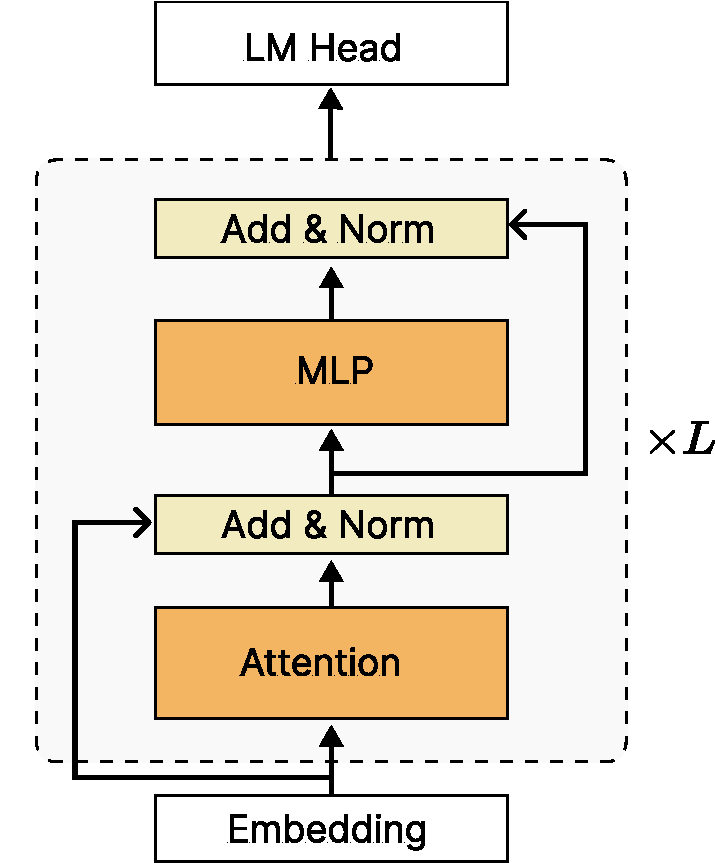
\includegraphics[width=0.75\linewidth]{figures/transformer.pdf}
    \caption{Decoder-only Transformer architecture.}
    \label{fig:decoder-only-transformer}
\end{figure}

\subsubsection{Attention}
The Transformer haven't introduced attention since we have seen that this has been used by Banhaudeau et al.,
in an RNN architecture. The innovation of Transformer is to remove the RNN and replace it fully with
\textbf{Mult-Head Attention (MHA)}. Given $\mathbf{X} \in \mathbb{R}^{T \times d_{\mathrm{model}}}$,
the sequence of token embeddings for $T$ positions, MHA projects the sequence into queries, keys
and values for $H$ heads:
\begin{equation}
    \mathbf{Q}, \mathbf{K}, \mathbf{V}
    \in \mathbb{R}^{T \times H \times d_{\mathrm{head}}}.
\end{equation}
Equivalently, each head $h$ has its own projections:
\begin{align}
    \mathbf{Q}_h &= \mathbf{X}\mathbf{W}^{Q}_h, &
    \mathbf{K}_h &= \mathbf{X}\mathbf{W}^{K}_h, &
    \mathbf{V}_h &= \mathbf{X}\mathbf{W}^{V}_h,
\end{align}
where $\mathbf{W}^{Q}_h \in \mathbb{R}^{d_{\mathrm{model}} \times d_q}$, 
$\mathbf{W}^{K}_h \in \mathbb{R}^{d_{\mathrm{model}} \times d_k}$
and $\mathbf{W}^{V}_h \in \mathbb{R}^{d_{\mathrm{model}} \times d_v}$ are learned projection
matrices for head $h$. The head output is then computed with scaled dot-product self-attention:
\begin{equation}
    \mathrm{head}_h
    =
    \mathrm{softmax}\left(
        \frac{\mathbf{Q}_h \mathbf{K}_h^\top + \mathbf{M}}{\sqrt{d_k}}
    \right)\mathbf{V}_h .
\end{equation}
For a decoder language model, $\mathbf{M}$ is a causal mask: entries corresponding to future
positions are set to $-\infty$, so token $i$ can only attend to tokens $j \leq i$. Multi-head attention runs $H$ such heads in parallel and concatenates their outputs:
\begin{equation}
    \mathrm{MHA}(\mathbf{X})
    =
    \mathrm{Concat}\left(\mathrm{head}_1,\ldots,\mathrm{head}_H\right)\mathbf{W}^{O},
\end{equation}
with $\mathbf{W}^{O} \in \mathbb{R}^{H d_v \times d_{\mathrm{model}}}$. Each head can therefore
learn a different projection of the same context, while the output projection mixes these views
back into the residual stream.

\text{\color{red} TODO: Linguistics specialization of heads}
\\
In standard MHA, as introduced in the original Transformer paper, the projection matrices
$\mathbf{W}^{Q}_h$, $\mathbf{W}^{K}_h$ and $\mathbf{W}^{V}_h$ are usually chosen so that all
heads together project back to a space of size $d_{\mathrm{model}}$. However, these projections
can become a bottleneck during generation. In a naive implementation, at each decoding step, all
previous tokens would be projected again to recompute their keys and values. The
\textbf{KV-Cache} reduces this computation and speeds up generation by caching the keys and values
of previous tokens. However, this cache grows linearly with the sequence length, and it is easy to
run out of memory when generating very long texts. To reduce the KV-Cache, we need to reduce the
dimensionality of keys and values.
\\
\text{\color{red} TODO: Redundancy of Heads and transition to GQA}

Among the popular approaches to reduce the KV-Cache, \textbf{Group Query Attention (GQA)}
shares key-value pairs to multiple query heads. Intuitively, the keys and values have fewer heads
than the queries:
\begin{align}
    \mathbf{K}, \mathbf{V} &\in \mathbb{R}^{T \times h_g \times h_{\mathrm{dim}}}, \\
    \mathbf{Q} &\in \mathbb{R}^{T \times h_q \times h_{\mathrm{dim}}},
    \qquad h_g < h_q .
\end{align}
The key-value heads are then broadcast to the query heads, and attention is computed as usual:
\begin{equation}
    \mathrm{Attention}(\mathbf{Q}, \mathbf{K}, \mathbf{V})
    =
    \mathrm{softmax}\left(\mathbf{Q}\mathbf{K}^{\top}\right)\mathbf{V}.
\end{equation}
Standard MHA corresponds to no sharing, while multi-query attention is the extreme case where all
query heads share the same keys and values. GQA is the compromise between the two: it reduces the
KV-Cache while keeping several different key-value heads.

While GQA reduces KV-cache memory, it does not reduce the attention computation. \textbf{Sparse Attention} reduces this compute 
by allowing each query to attend to only a subset of previous tokens. 
DeepSeek Sparse Attention \cite{deepseekai2025deepseekv32pushingfrontieropen} introduces a lightweight \textit{lightning indexer} 
that cheaply scores all previous tokens using a small number of low-dimensional attention heads. 
The top-k scoring keys are then selected, and the expensive main attention is computed only 
over those key-value entries. The main attention therefore changes from $\mathcal{O}(L^2)$ to $\mathcal{O}(Lk)$, 
where $k \ll L$ is the number of selected tokens. The indexer itself remains $\mathcal{O}(L^2)$, 
but its constant cost is much smaller because it uses very small dimensions, few heads, 
and FP8 computation. 
\begin{figure}[!htbp]
    \centering
    \subfloat[DeepSeek Sparse Attention.]{
        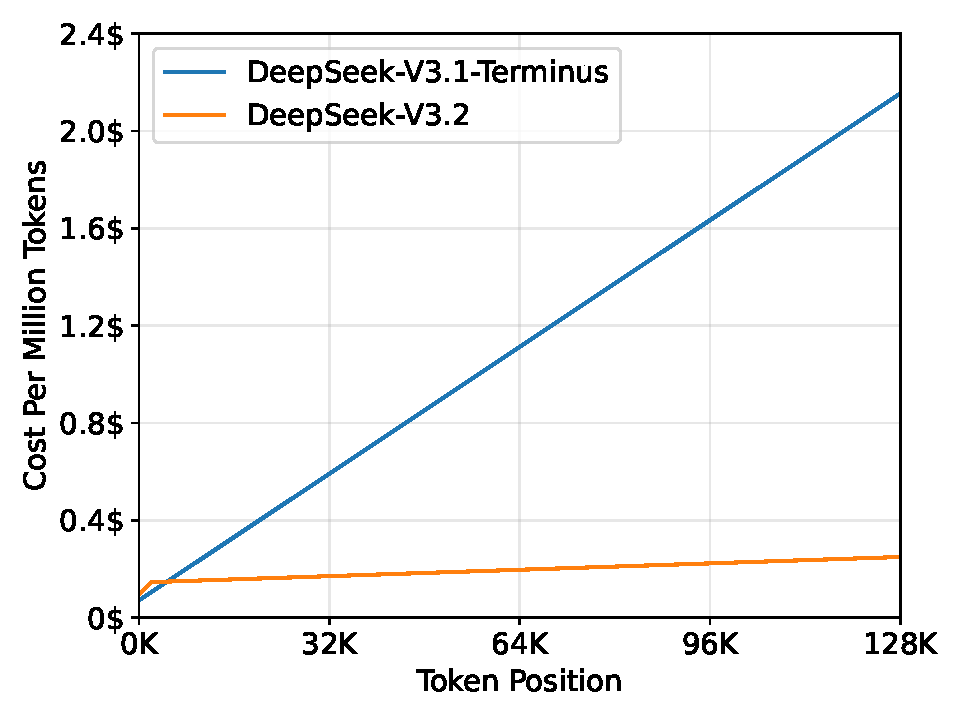
\includegraphics[width=0.70\linewidth]{figures/cost_decoding.pdf}
    }
    \\[0.5em]
    \subfloat[Sliding Window Attention.]{
        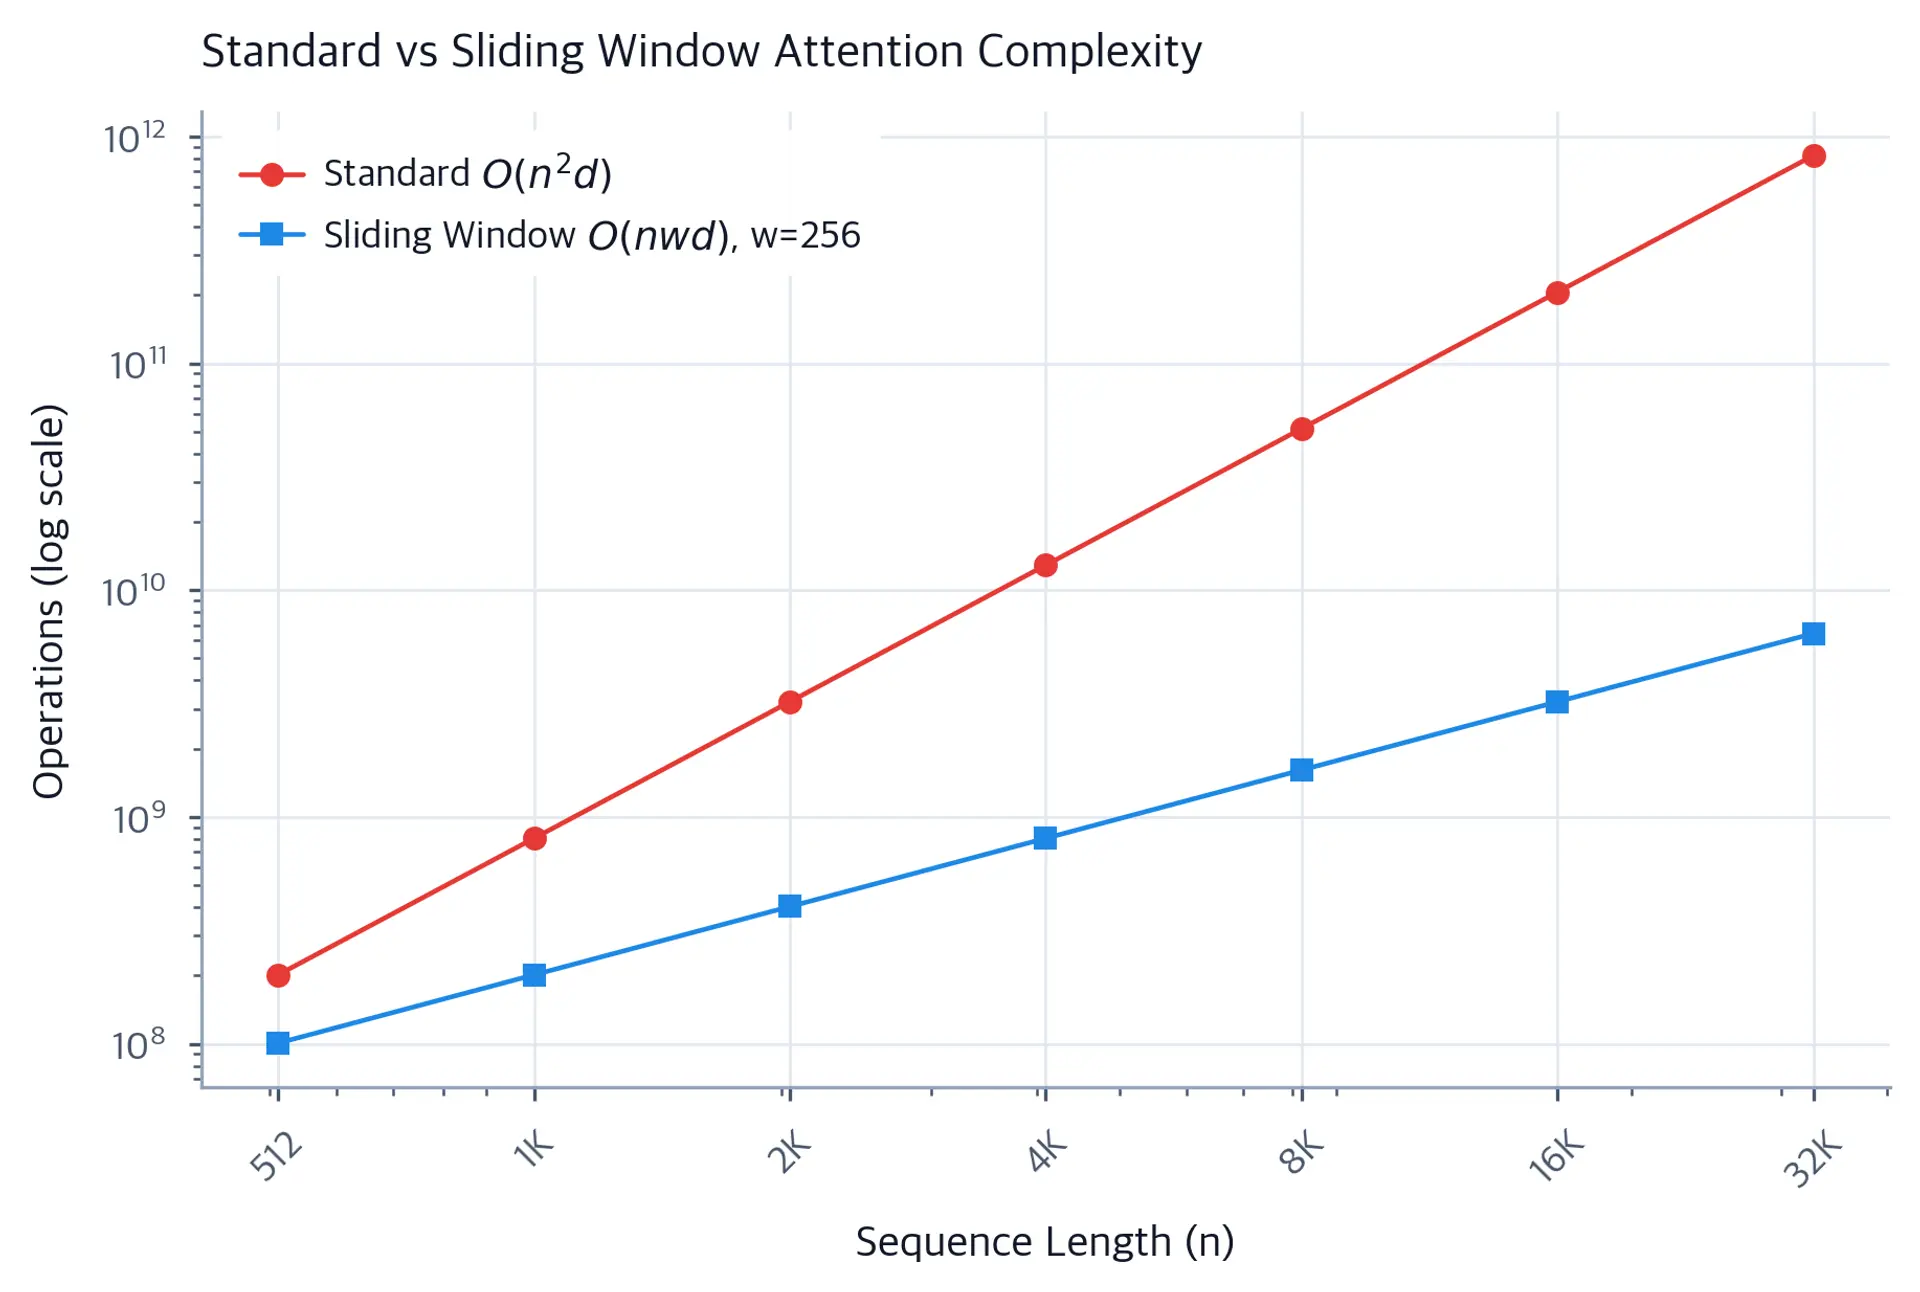
\includegraphics[width=0.70\linewidth]{figures/sliding-window-complexity-comparison-1920w.png}
    }
    \caption{Sparse-attention decoding costs and computation savings. (a) DeepSeek Sparse Attention (DeepSeek-v3.2) vs DeepSeek with full attention (DeepSeek-v3.1-Terminus) \cite{deepseekai2025deepseekv32pushingfrontieropen}. (b) How Sliding Window Attention reduces computation, from https://mbrenndoerfer.com/writing/sliding-window-attention}
    \label{fig:sparse-attention-costs}
\end{figure}
While many recent models use a derivative of DeepSeek Sparse Attention (cite Qwen, GLM), 
it is not the first work to introduce sparse attention (\textit{TODO: Attention Sink}),
which has been widely studied \cite{kitaev2020reformer,roy2021routing,beltagy2020longformer,tang2024quest}. 
Sliding-Window Attention is a simple form of sparse attention where each query attends only 
to a fixed number of nearby tokens instead of the entire preceding sequence. 
For a query at position $i$ and a window size $w$, attention is restricted 
to the key-value pairs ${(k_{i-w},v_{i-w}),\ldots,(k_i,v_i)}$.
Each query therefore attends to only $w$ tokens rather than all $L$ previous tokens, 
reducing the attention complexity from $O(L^2)$ to $O(Lw)$, where typically $w \ll L$. 
This saves compute and save KV-Cache memory if the implementation discards KV 
states that fall outside the active window
Sliding-window attention benefits from model depth because information can propagate 
from one local window to another across successive layers, even though attention is local 
within each individual layer. However, long-range information is accessed only indirectly 
through model depth, whereas full attention allows a query to directly attend to any previous 
token at each layer. For this reason, many LLMs use hybrid architectures that combine local-attention 
layers with occasional full-attention layers 
\cite{gemmateam2024gemma2improvingopen,gemmateam2025gemma3technicalreport,gemmateam2026gemma4technicalreport}.
Many of the efficient attentions methods are orthogonal to each other, so they can be combined. For example,
it is possible to combine sparse attention with local attention and sliding window attention. Or just as DeepSeek-v4
combine sparse attention with multi-latent attention which is another method for learning compressed kv-cache
during pre-training.

\subsubsection{Multilayer Perceptron}
After the attention layer, the conetextualized tokens are fed into the Multilayer Perceptron (MLP). While attention is a token-mixing operation, the MLP is a channel-mixing operation, each token is forwarded independantly into the MLP. In the original Transformer's paper, the MLP is defined as:
$$
\text{MLP}(x) = f(\textbf{x}\textbf{W}_{up})\textbf{W}_{down}
$$
where $f(\cdot)$ is the non-linear activation function, 
$\textbf{W}_{\text{up}} \in \mathbb{R}^{d_{\text{model}} \times d_{\text{inter}}}$ 
project the input token $\mathbf{x} \in \mathbb{R}^{d_{\text{model}}}$ in higher dimension, 
with $d_{\text{model}} \ll d_{\text{inter}}$. And finally, $\textbf{W}_{\text{down}} \in \mathbb{R}^{d_{\text{inter}} \times d_{\text{model}}}$,
projects backs to the model dimension.
Modern LLMs often replace this simple MLP with a gated linear unit variant. Instead of applying
only one non-linearity to the expanded representation, the block learns two projections: one
projection $\mathbf{V}_{\text{up}}$ produces the values, and the other projection
$\mathbf{W}_{\text{up}}$ gates them. Omitting bias terms, these alternatives can be written as:
\begin{align}
    \mathrm{MLP}_{\mathrm{GLU}}(\mathbf{x})
    &= \left(\sigma(\mathbf{x}\mathbf{W}_{\text{up}}) \odot \mathbf{x}\mathbf{V}_{\text{up}}\right)\mathbf{W}_{\text{down}}, \\
    \mathrm{MLP}_{\mathrm{GEGLU}}(\mathbf{x})
    &= \left(\mathrm{GELU}(\mathbf{x}\mathbf{W}_{\text{up}}) \odot \mathbf{x}\mathbf{V}_{\text{up}}\right)\mathbf{W}_{\text{down}}, \\
    \mathrm{MLP}_{\mathrm{Bilinear}}(\mathbf{x})
    &= \left(\mathbf{x}\mathbf{W}_{\text{up}} \odot \mathbf{x}\mathbf{V}_{\text{up}}\right)\mathbf{W}_{\text{down}}, \\
    \mathrm{MLP}_{\mathrm{SiLU}}(\mathbf{x})
    &= \left(\mathrm{SiLU}(\mathbf{x}\mathbf{W}_{\text{up}}) \odot \mathbf{x}\mathbf{V}_{\text{up}}\right)\mathbf{W}_{\text{down}}, \\
    \mathrm{MLP}_{\mathrm{ReGLU}}(\mathbf{x})
    &= \left(\mathrm{ReLU}(\mathbf{x}\mathbf{W}_{\text{up}}) \odot \mathbf{x}\mathbf{V}_{\text{up}}\right)\mathbf{W}_{\text{down}}.
\end{align}
Here $\odot$ denotes element-wise multiplication. \ref{tab:gated_mlp} gives the performance of each activation on SuperGLUE benchmark. 
We can see that SiLU activation gives better results, this explains why many LLMs use it as activations: Mistral-v0.1, Granite, etc.
\begin{table*}[h!]
    \centering
    \setlength{\tabcolsep}{8pt}
    \begin{tabular}{>{\raggedright\arraybackslash}p{0.30\textwidth}>{\centering\arraybackslash}p{0.40\textwidth}}
        \toprule
        \textbf{} & \textbf{Average SuperGLUE score} \\
        $\mathrm{MLP}_{\mathrm{GLU}}$ & 73.95 \\
        $\mathrm{MLP}_{\mathrm{GEGLU}}$ & 73.96 \\
        $\mathrm{MLP}_{\mathrm{Bilinear}}$ & 73.81 \\
        \rowcolor[HTML]{EEE0CC}$\mathrm{MLP}_{\mathrm{SwiGLU}}$ & \textbf{74.56} \\
        $\mathrm{MLP}_{\mathrm{ReGLU}}$ & 73.66 \\
        \bottomrule
    \end{tabular}
    \caption{Average SuperGLUE score for gated MLP variants.}
    \label{tab:gated_mlp}
\end{table*}
It is difficult to explain why gated MLP with work better with some activations than other. 
Citing \citet{shazeer2020gluvariants}, the author of gated MLPs:
\begin{quote}
    \small\itshape
    ``We offer no explanation as to why these architectures seem to work; we attribute their
    success, as all else, to divine benevolence.''

    \begin{flushright}
    \normalfont--- Noam Shazeer, \textit{GLU Variants Improve Transformer (2020)}
    \end{flushright}
\end{quote}
In modern LLM architectures, the MLP parameters can occupy over to $90\%$ of the total model parameters. 
It has been shown that MLP layers play an important role in storing knowledge acquired during web-scale pretraining. 
\citet{geva-etal-2021-transformer} interpret the MLP as a key--value memory:
each column of \(\mathbf{W}_{\text{up}}\) in the MLP represents a key
\(\mathbf{k}_i\) that detects linguistic patterns seen during training, while
each row of \(\mathbf{W}_{\text{down}}\) represents the corresponding value
\(\mathbf{v}_i\), which promotes the tokens likely to follow those patterns.
The key \(\mathbf{k}_i\) can be strongly or weakly activated depending on the
input \(x\). When \(\mathbf{k}_i\) is strongly activated, its corresponding
value \(\mathbf{v}_i\) is assigned a large weight and therefore contributes
more strongly to the MLP output. This mechanism can be schematized as follows:
\[
\boxed{
\underbrace{\mathbf{k}_i(\mathbf{x})}_{
    \text{whether the key's pattern is active}
}
\;\longrightarrow\;
\underbrace{\mathbf{v}_i}_{
    \text{promotes tokens likely to follow the pattern}
}
}
\]
\begin{table*}[t]
    \centering
    \small
    \setlength{\tabcolsep}{6pt}
    \renewcommand{\arraystretch}{1.15}

    \begin{tabularx}{\textwidth}{@{} l l c >{\raggedright\arraybackslash}X @{}}
        \toprule
        \textbf{Value}
        & \textbf{Top prediction}
        & \textbf{Precision@50}
        & \textbf{Matching trigger example} \\
        \midrule

        $\mathbf{v}^{15}_{222}$
        & \emph{each}
        & 68\%
        & \emph{But when bees and wasps resemble \textcolor{blue}{each}} \\

        \midrule

        $\mathbf{v}^{16}_{752}$
        & \emph{played}
        & 16\%
        & \emph{Her first role was in Vijay Lalwani's psychological thriller
        Karthik Calling Karthik, where Padukone was cast as the supportive
        girlfriend of a depressed man (\textcolor{blue}{played}} \\

        \midrule

        $\mathbf{v}^{13}_{2601}$
        & \emph{extratropical}
        & 4\%
        & \emph{Most of the winter precipitation is the result of synoptic-scale,
        low-pressure weather systems (large-scale storms such as
        \textcolor{blue}{extratropical}} \\

        \midrule

        $\mathbf{v}^{15}_{881}$
        & \emph{part}
        & 92\%
        & \emph{Comet served only briefly with the fleet, owing in large
        \textcolor{blue}{part}} \\

        \midrule

        $\mathbf{v}^{16}_{2070}$
        & \emph{line}
        & 84\%
        & \emph{Sailing from Lorient in October 1805 with one ship of the
        \textcolor{blue}{line}} \\

        \midrule

        $\mathbf{v}^{12}_{3186}$
        & \emph{jail}
        & 4\%
        & \emph{On May 11, 2011, four days after scoring 6 touchdowns for the
        Slaughter, Grady was sentenced to twenty days in
        \textcolor{blue}{jail}} \\

        \bottomrule
    \end{tabularx}

    \caption{
    Examples of MLP key--value memory pairs identified by
    \citet{geva-etal-2021-transformer}.
    For each value vector $\mathbf{v}^{\ell}_{i}$, \emph{Top prediction}
    is the vocabulary token receiving the highest score when the value is
    projected through the model's output embedding.
    \emph{Precision@50} is the percentage of the 50 training prefixes that
    most strongly activate the paired key $\mathbf{k}^{\ell}_{i}$ whose
    ground-truth next token equals that prediction.
    The final column presents one such matching prefix, with its
    ground-truth next token shown in blue.
    }
    \label{tab:ffn-key-value-examples}
\end{table*}
The MLP does not only store lexical knowledge. At some point, this lexical knowledge coincides 
with factual knowledge. When a key detecting the prefix \textit{The capital of France is} 
is strongly associated with a value representing \textit{Paris}, this lexical key--value memory 
turns out to also encode world knowledge. 
Hence, more broadly, it is widely believed that MLPs play a central role in storing the knowledge acquired during pretraining
\citet{geva-etal-2021-transformer,dai-etal-2022-knowledge}.
This view is also reflected in many knowledge-editing methods, which often directly target MLP weights
\citet{meng2023locatingeditingfactualassociations,meng2023masseditingmemorytransformer, fang2025alphaeditnullspaceconstrainedknowledge}.

\subsubsection{Language Modeling Head}
Well, the tokens are contextualized thanks to the multi-head attention, and each token retrieves 
the relevant knowledge encoded within the MLP. This process is repeated for $L$ layers and at the end
produces a context vector $\textbf{c}$ that is ready for next token prediction 
using the language modeling head (LM Head or output embedding).
The LM Head is another important component in large scale Transformer LLM. First, the token vocabulary becames quite
large due to the diversity of tokens that can be infered from a web scale data. Hence, the LM Head weight can occupy
a huge amount of parameters in the LLM, particulary for small LLMs. Figure \ref{fig:emb-param-ratio} shows the memory
occupied by the input/output embedding parameters for different model sizes, including dense and quantized ones.
We can see that the embedding and LM Head parameters represent a larger fraction of the model 
when the Transformer backbone is small\footnote{Quantization is usually not applied to the embedding weights.}.
\begin{figure}[ht]
    \centering
    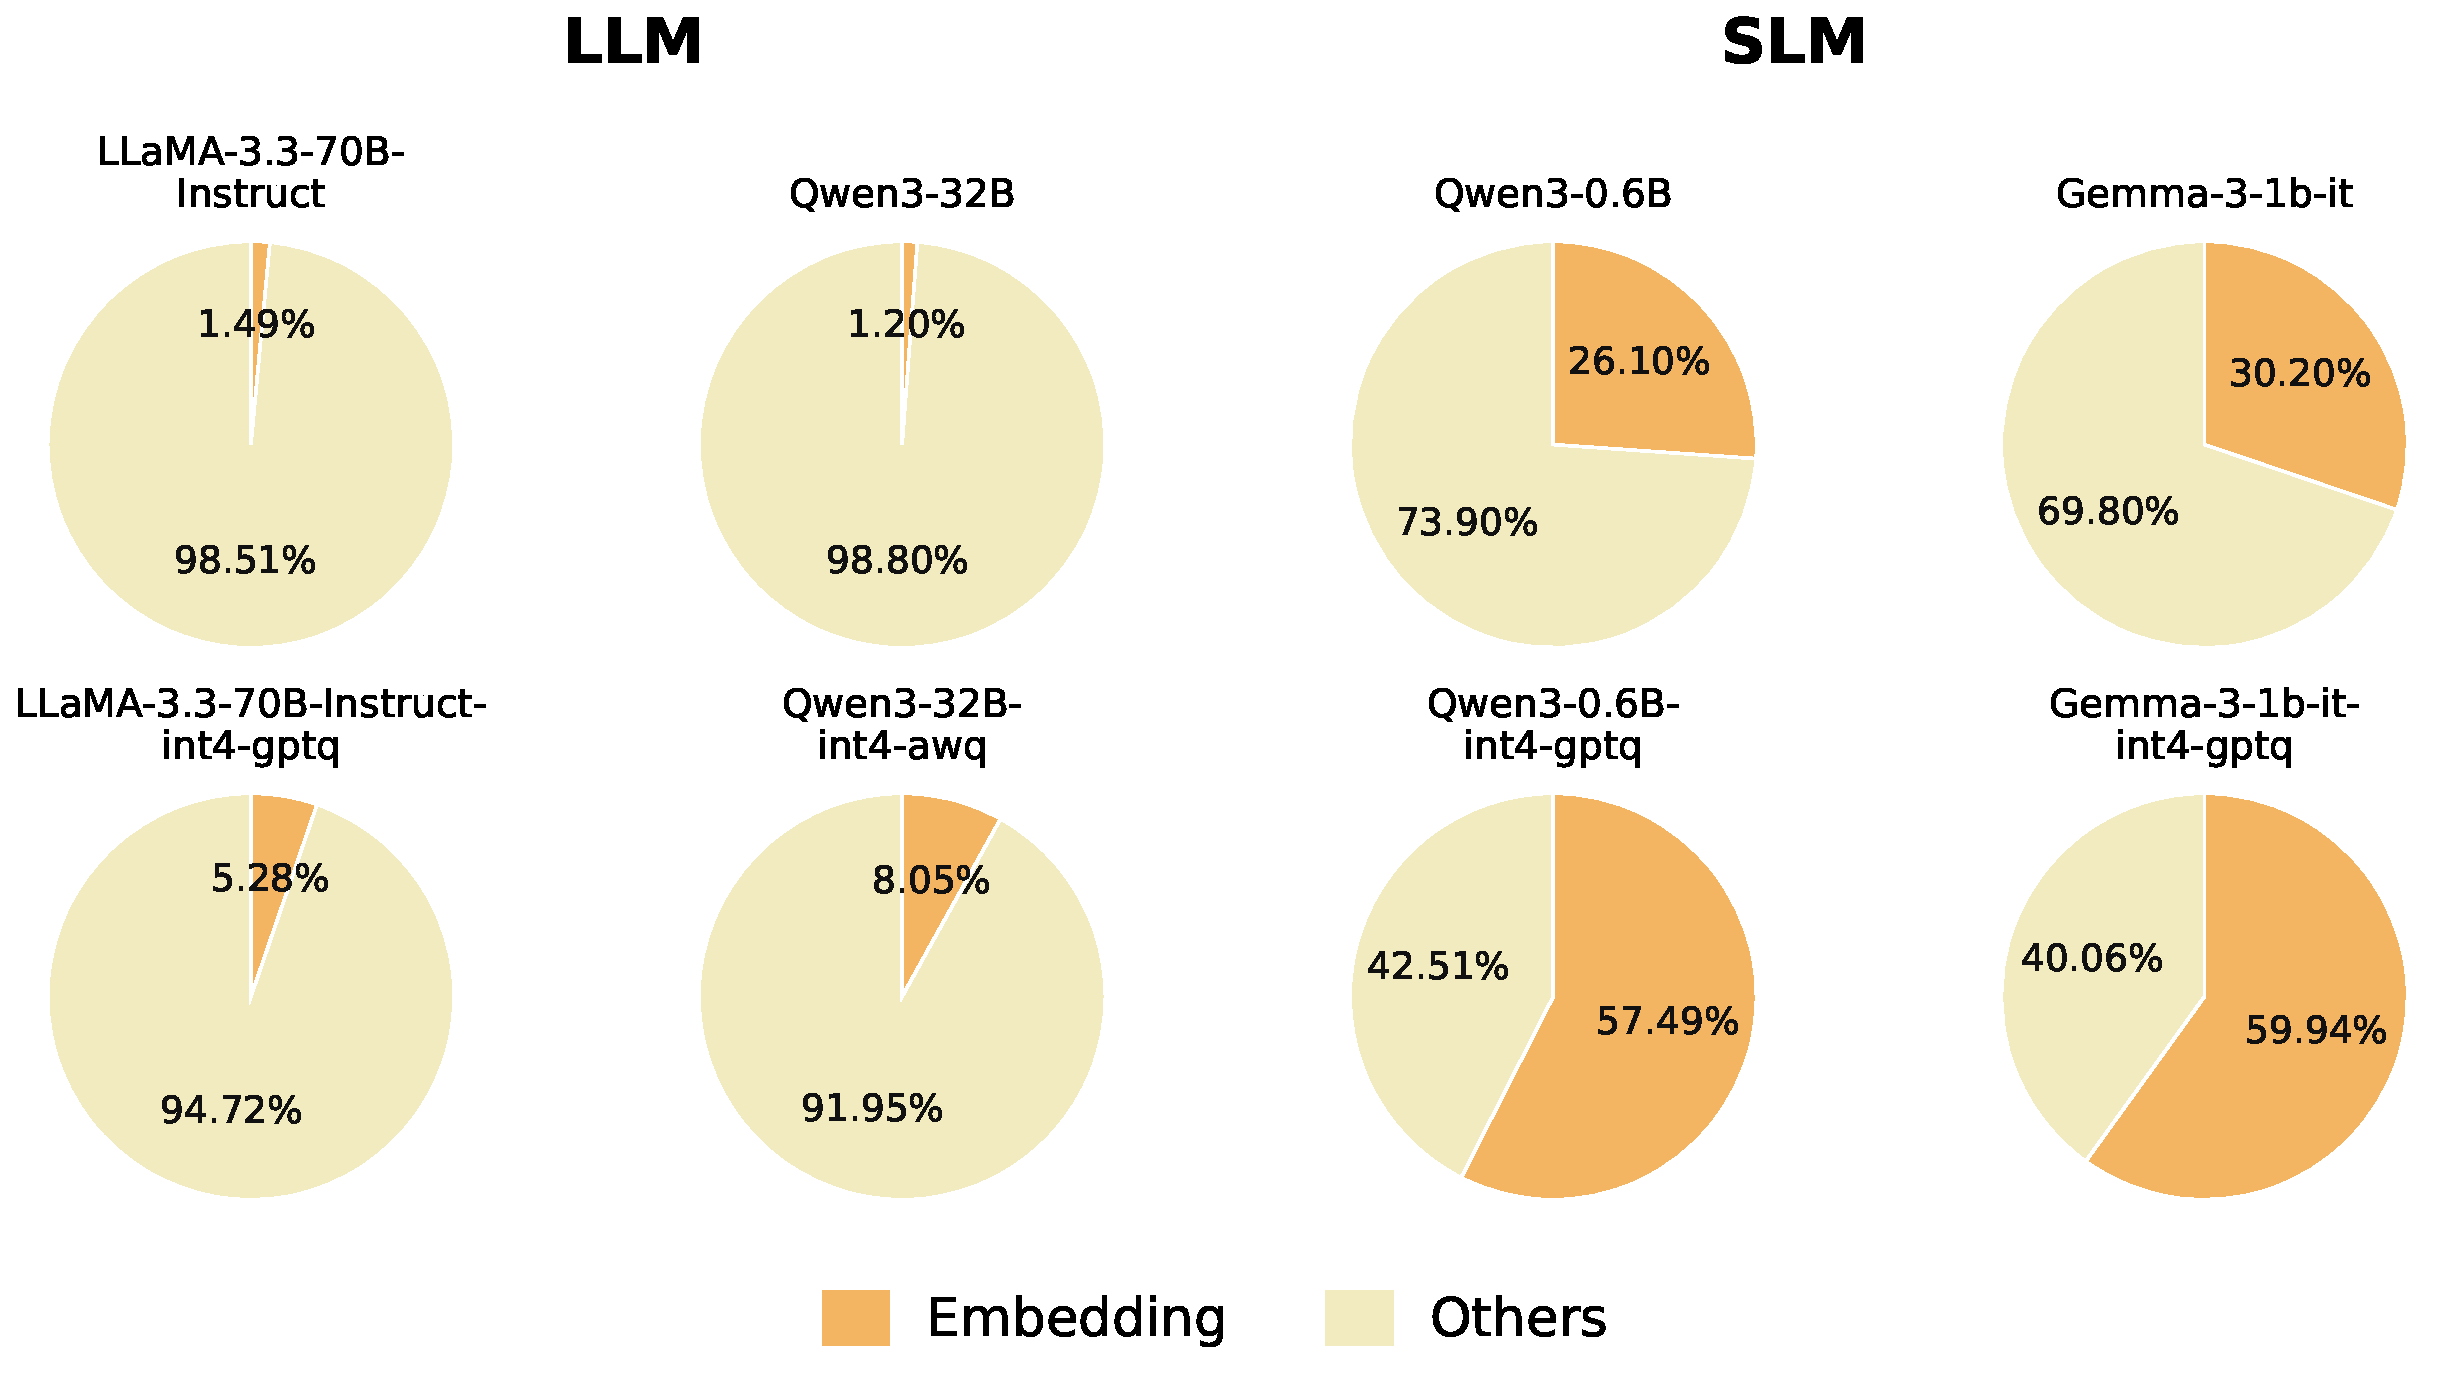
\includegraphics[width=1.0\linewidth]{figures/embedding_parameter_ratio.pdf}
    \caption{Proportion of the size in MB of embedding parameters across different model sizes.
    Data taken from \href{https://blog.squeezebits.com/vocabulary-trimming-methods}{https://blog.squeezebits.com/vocabulary-trimming-methods}.}
    \label{fig:emb-param-ratio}
\end{figure}
This is mainly caused by the large vocabulary of the models. A common solution to reduce the size by half is
weight tying, which shares the input and output embedding. Almost all small LLMs use weight tying, which haven't
proven to hurt parameters, while still reducing a lot the model's parameters.

Another approach to reducing the number of parameters occupied by the LM head
is to factorize its weight matrix into two low-rank matrices. This strategy was
notably adopted in ALBERT~\citep{lan2020albertlitebertselfsupervised}, where
the embedding dimension was reduced from $768$ to $128$ without sacrificing downstream performance. 
More precisely, given the input $\mathbf{x}\in\mathbb{R}^{d}$ and an LM-head weight
matrix $\mathbf{W}\in\mathbb{R}^{d\times V}$, the factorized projection is
\begin{equation}
    \mathbf{x}\mathbf{W}
    \quad\longrightarrow\quad
    (\mathbf{x}\mathbf{W}_1)\mathbf{W}_2,
\end{equation}
where $\mathbf{W}_1\in\mathbb{R}^{d\times r}$,
$\mathbf{W}_2\in\mathbb{R}^{r\times V}$, and $r\ll H$. This reduces the
LM-head parameter count from $dV$ to $dr+rV$.

However, some works have identified what is known as the
\textit{softmax bottleneck}~\citep{yang2018breakingsoftmaxbottleneck}:
a low-dimensional LM head can only produce a limited variety of output
distributions. Therefore, reducing its rank too aggressively can limit the
model's ability to predict complex token distributions. \citet{godey2024smalllanguagemodelsunderperform}
studied this by compressing the LM Head rank dimension at different sizes and found that smaller rank
hurts performance and limits the expressiviness of the probability distribution as shown in Figure \ref{fig:lm_head_botlnck}. 
More importantly, this also hurts the learning signal during training \citet{godey2026lostbackpropagationlmhead}.
There are many solutions to avoid the \textit{softmax bottleneck}. Since this phenomen arises mainly when
$r \ll V$, an obvious solution is to augment $r$ or $V$ the voabulary size. Reducing the vocabulary size can be
achieve by using a tokenizer with few tokens or falling back to a character or bytes tokenizers.
It is also technically possible after training to remove tokens in the input/embedding embedding.
But this is risky as it can affect critical tokens. This discussion is releated to the research we will present
later, which proposes to reduce the rank of the LM Head instead of pruning tokens in multilingual transformer models.
\begin{figure}[ht]
    \centering
    \subfloat[Accuracy.]{
        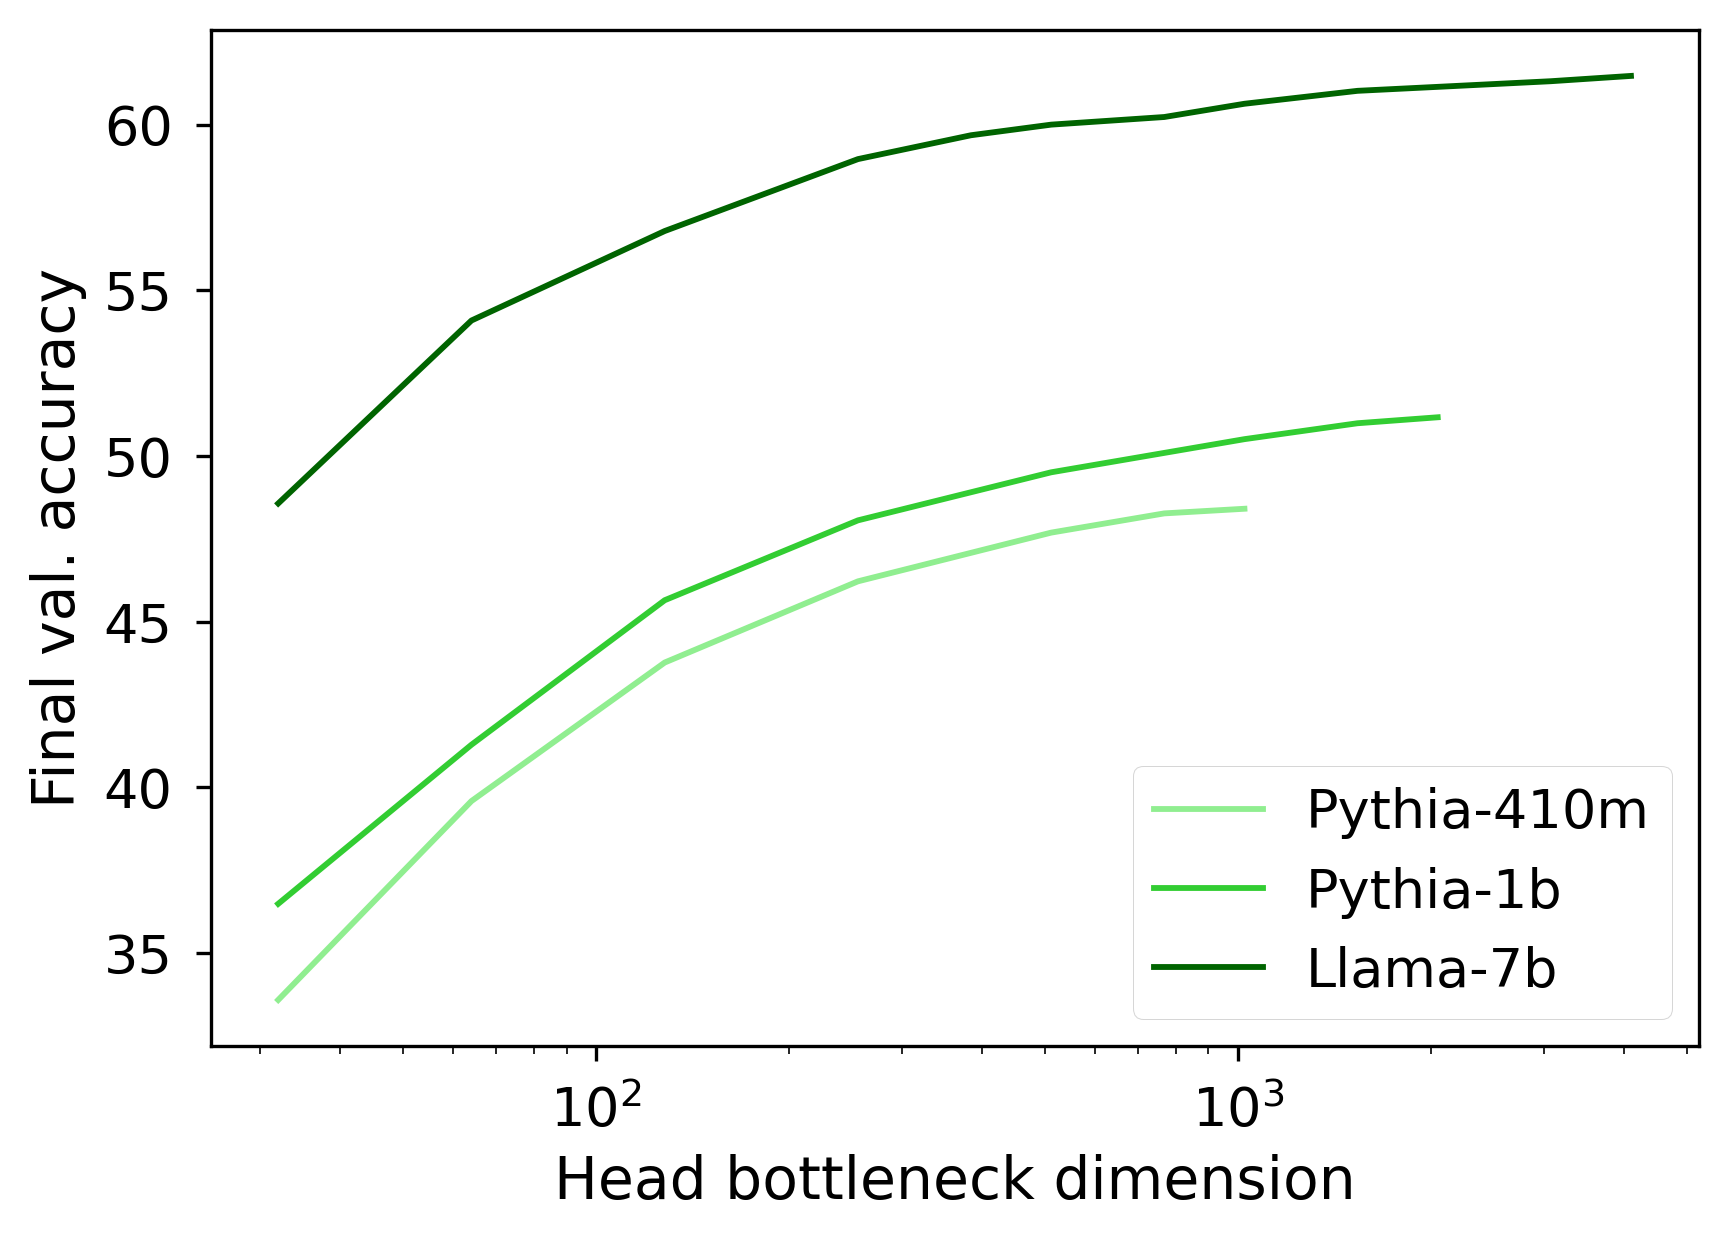
\includegraphics[width=0.48\linewidth]{figures/figure6_accuracy.png}
    }
    \hfill
    \subfloat[Cross-entropy.]{
        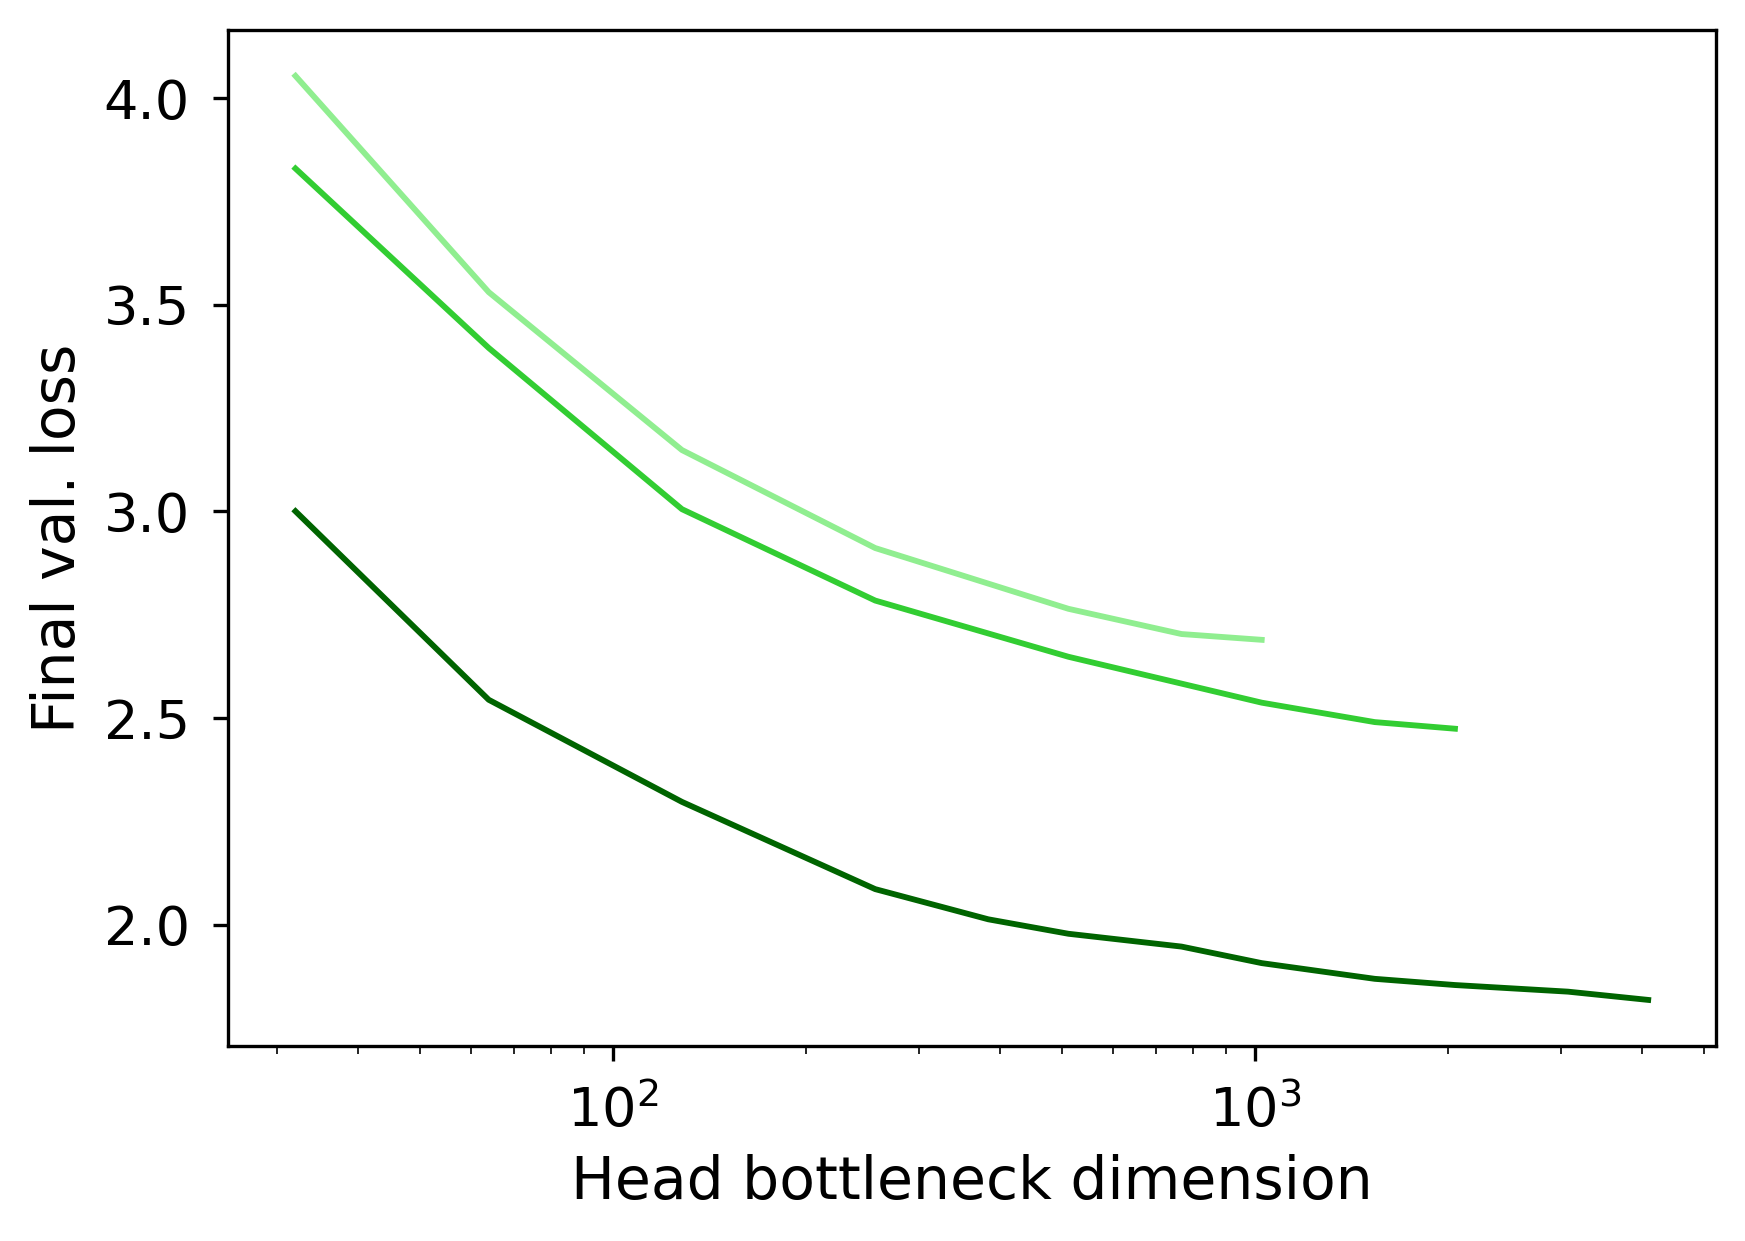
\includegraphics[width=0.48\linewidth]{figures/figure6_cross_entropy.png}
    }
    \caption{Effect of reducing the LM Head rank on accuracy and cross-entropy.
    Figures from \citet{godey2024smalllanguagemodelsunderperform}.}
    \label{fig:lm_head_botlnck}
\end{figure}

\subsection{A Transformer is never enough large}
What made the Transformer architecture particularly successful in language
modeling is its ability to scale both the number of parameters and the amount
of training data. Since Transformer training can be efficiently parallelized
across multiple GPUs, increasingly large models can be trained on increasingly
large datasets, leading to improved performance and the emergence of new
capabilities. However, scaling cannot be done blindly: given the high cost of
pretraining, the allocation between model size and training data must be
estimated before the final training run. For a fixed compute budget, how large
should the model be, and on how many tokens should it be trained?

Denoting the number of parameters by $N$, the number of training tokens by $D$,
and the training compute by $C$, the compute cost of a dense Transformer can be
approximated as $C \approx 6ND$. So given a training budget $C$ fixed 
(how many training flops is available for training), how much
the model size should take in this compute and how much the training tokens should take in this budget.
Both Kaplan \cite{kaplan2020scaling} and Chinchilla \cite{hoffmann2022training} 
scaling find that the compute-optimal model size and dataset size  follow power laws 
in the compute budget: $N_{\mathrm{opt}} \propto C^{\alpha}$ and $D_{\mathrm{opt}} \propto C^{\beta}$.
\textbf{Kaplan scaling laws} estimate that the compute-optimal allocation with 
$N_{\mathrm{opt}} \propto C^{0.73}$ and  $D_{\mathrm{opt}} \propto C^{0.27}$.
Thus, model size should increase much faster than training data, 
which favors very large models trained on comparatively few tokens. 
On the other side, the \textbf{Chinchilla scaling laws}
later find that model size and training data should instead scale approximately equally:
$N_{\mathrm{opt}} \propto C^{0.5}$ and $D_{\mathrm{opt}} \propto C^{0.5}$. Since Kaplan and Chinchila
scaling laws, lot of types scaling laws are proposed for training LLMs. 
Often it is about adding new scaling axis such as sparsity and granularity in the case 
of sparse Transformer model. It can also be about accounting a constrain such as an inference budget.

Beyond guiding compute allocation, scaling laws also reveal how model capabilities
evolve with scale. While performance often improves predictably as training compute
increases, some abilities appear only after the model reaches a certain scale. The
model may remain close to random performance across several scales before suddenly
crossing a plateau and acquiring a new ability. \citet{wei2022emergent} identify
several such \textit{emergent abilities}.
\begin{figure}[ht]
    \centering
    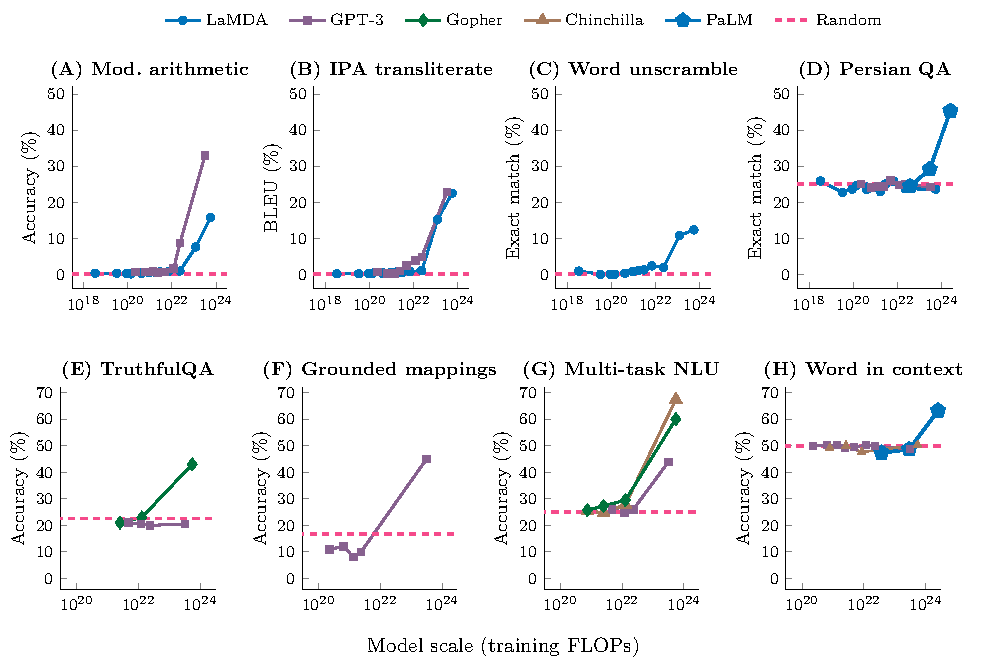
\includegraphics[width=1.0\linewidth]{figures/wei_emergent_abilities_figure.pdf}
    \caption{Examples of emergent abilities in large language models.
    Figure from \citet{wei2022emergent}. 
    A capacity is emergent when the score surpasses the random baseline 
    while it wasn't at smaller scale.}
    \label{fig:wei-emergent-abilities}
\end{figure}

Then a question arises. Is there a point beyond which increasing the number of parameters no longer
produces meaningful improvements? Testing this hypothesis directly is difficult,
since training models at the largest scales is extremely costly.
Classical scaling laws predict \textit{diminishing returns}: test loss continues
to decrease with scale, but each additional increase in model size produces a
smaller improvement~\citep{kaplan2020scaling,hoffmann2022training}. However,
whether this implies diminishing returns in model capabilities depends on how
performance is measured. \citet{sinha2026illusion} argue that short-task
benchmarks may create an illusion of saturation. Even small improvements in
single-step accuracy can compound into large improvements in the length of tasks
that a model can reliably execute. Therefore, diminishing returns on loss or
short-task accuracy do not necessarily imply diminishing returns in practical
capabilities.
